\documentclass{math}

\usepackage{float}
\usepackage{graphicx}
\usepackage{subcaption}
\geometry{letterpaper, margin=0.8in}

\title{Principles of Data Mining: HW 08}
\author{Alvin Lin}
\date{August 2018 - December 2018}

\begin{document}

\maketitle

\subsection*{Question 1}
Why do we use 10 visits instead of just keeping records of every single visit?
\par
We sum up 10 visits into a single data point to reduce the variance between
each visit and also to exaggerate their purchase patterns by accumulating their
most common purchases into a single data point. Summing 10 visits from a guest
creates a representative data point of that guest.

\subsection*{Question 5}
\begin{figure}[H]
  \centering
  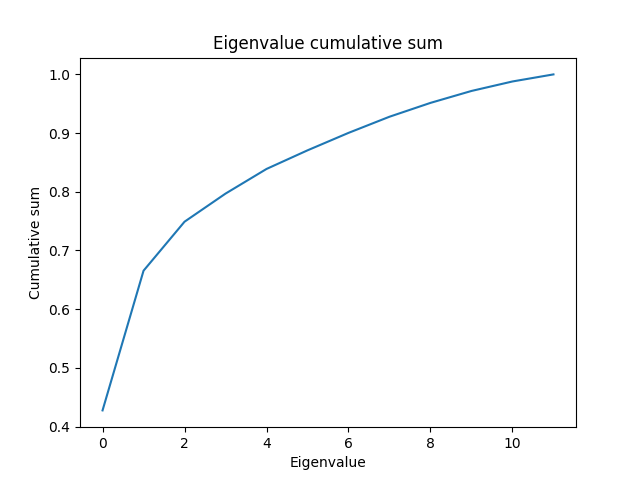
\includegraphics[width=15cm]{assets/hw_08_eigenvalue_cumsum.png}
  \caption{Cumulative sum of the eigenvalues sorted greatest to least}
\end{figure}

\subsection*{Question 6}
Two largest eigenvectors:
\begin{center}
  \scalebox{0.9}{\begin{tabular}{|c|c|c|c|c|c|c|c|c|c|c|c|}
    \hline
    Milk & PetFood & Veggies & Cereal & Bread & Rice & Meat & Eggs & Yogurt &
      Chips & Cola & Fruit \\
    \hline
    0.124 & 0.259 & -0.353 & 0.294 & 0.247 & -0.349 & -0.031 & -0.004 & -0.385 &
      0.319 & 0.375 & -0.363 \\
    -0.492 & -0.242 & -0.151 & -0.362 & -0.368 & -0.275 & 0.47 & 0.004 &
      -0.073 & 0.246 & 0.22 & 0.006 \\
    \hline
  \end{tabular}}
\end{center}
The eigenvectors tell us the amount of variance along a specific dimension.
The first eigenvector shows high relative variance along veggies, rice, yogurt,
chips, and cola. The second eigenvector shows us high relative variance for
milk, cereal, and bread. This tells us the spread of the data when we project it
onto the two eigenvectors.

\subsection*{Question 7}
Project the original agglomeration data onto these first two eigenvectors:
\begin{figure}[H]
  \begin{subfigure}{0.5\linewidth}
    \centering
    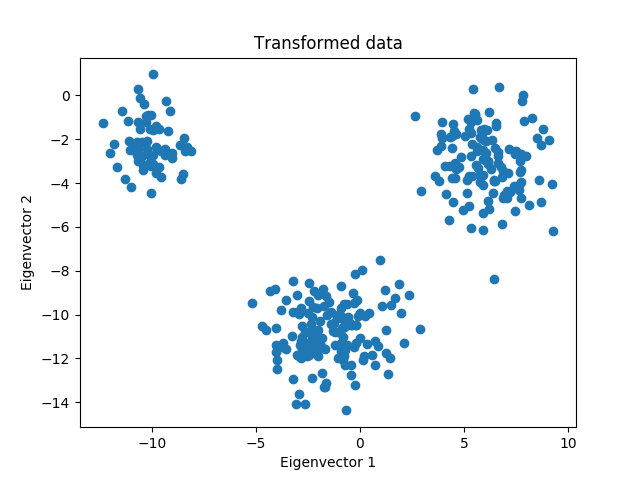
\includegraphics[width=9cm]{assets/hw_08_projected_data.png}
    \caption{Data projected onto eigenvectors}
  \end{subfigure}
  \begin{subfigure}{0.5\linewidth}
    \centering
    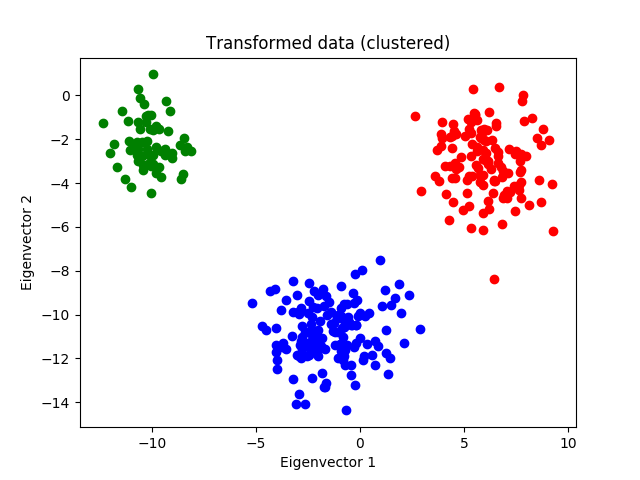
\includegraphics[width=9cm]{assets/hw_08_projected_data_clustered.png}
    \caption{Data projected onto eigenvectors (clustered)}
  \end{subfigure}
\end{figure}

\subsection*{Question 8}
Find the center of mass of each of the \( k \) clusters that you got out of
KMeans. These are 2D vectors.
\begin{center}
  \begin{tabular}{|c|c|c|}
    \hline
    & Eigenvector 1 & Eigenvector 2 \\
    \hline
    Center 1 & 6.093 & -3.024 \\
    Center 2 & -10.104 & -2.213 \\
    Center 3 & -1.449 & -10.786 \\
    \hline
  \end{tabular}
\end{center}
These centers of mass are the cluster prototypes projected on this 2D
eigenvector space.

\subsection*{Question 9}
Multiply these centers of mass back times the first two eigenvectors.
\begin{center}
  \scalebox{0.9}{\begin{tabular}{|c|c|c|c|c|c|c|c|c|c|c|c|c|}
    \hline
    Milk & PetFood & Veggies & Cereal & Bread & Rice & Meat & Eggs & Yogurt &
      Chips & Cola & Fruit \\
    \hline
    2.24 & 2.31 & -1.69 & 2.89 & 2.62 & -1.30 & -1.61 & -0.03 & -2.13 & 1.20 &
      1.62 & -2.23 \\
    -0.16 & -2.08 & 3.90 & -2.17 & -1.69 & 4.13 & -0.73 & 0.03 & 4.05 & -3.76 &
    	-4.27	& 3.66 \\
    5.12 & 2.23 & 2.14 & 3.47 & 3.61 & 3.47 & -5.03 & -0.03 & 1.34 & -3.12 &
    	-2.91	& 0.46 \\
    \hline
  \end{tabular}}
\end{center}
The relative amounts of each item bought indicate the shopping preferences of
that cluster. These are a bit strange since some items contain negative amounts
which doesn't make sense. I attempted to ``normalize'' the data by shifting all
the prototypes in the positive direction so that no value was negative:
\begin{center}
  \scalebox{0.9}{\begin{tabular}{|c|c|c|c|c|c|c|c|c|c|c|c|c|}
    \hline
    Milk & PetFood & Veggies & Cereal & Bread & Rice & Meat & Eggs & Yogurt &
      Chips & Cola & Fruit \\
    \hline
    4.47 & 4.54 & 0.54 & 5.12 & 4.85 & 0.94 & 0.62 & 2.20 & 0.10 & 3.43 &
      3.85 & 0.00 \\
    4.11 & 2.19 & 8.17 & 2.10 & 2.58 & 8.40 & 3.54 & 4.30 & 8.32 & 0.51 &
      0.00 & 7.93 \\
    10.15 & 7.26 & 7.17 & 8.50 & 8.63 & 8.49 & 0.00 & 4.99 & 6.37 & 1.91 &
      2.11 & 5.49 \\
    \hline
  \end{tabular}}
\end{center}
I'm not entirely sure if this is more or less informative. Unlike the results
we obtained from hierarchical agglomeration, we can no longer distinctively see
a ``party animal'' cluster prototype from these clusters.

\subsection*{Question 10}
The first thing we did was find the covariance matrix and take its eigenvectors,
which determines the most significant dimensions (the ones with the most
variance). This gives us a series of eigenvectors which we can project the data
onto to reduce its dimensionality and make sense of it. By ordering the
eigenvectors by eigenvalue from high to low and projecting the data onto it, we
reduce the data to 2 dimensions and stretch it along the attributes that matter
the most. By inspection, we can see that this new data has 3 distinct clusters,
which we can separate out using the KMeans clustering algorithm with
\( k = 3 \). \par
I almost made the same mistake that I did in HW 06 by forgetting to remove the
ID attribute. The projection of the data onto the two eigenvectors (including
the ID field) still looked viable, since there were also three relatively
distinct clusters. The cluster prototypes obtained from principal component
analysis are very different from those obtained by hierarchical agglomeration.
This is likely due to the fact that dimensional reduction tends to cause a loss
of precision and information.

\begin{center}
  If you have any questions, comments, or concerns, please contact me at
  alvin@omgimanerd.tech
\end{center}

\end{document}
